\documentclass[11pt]{article}

% ---------------------------------------------------------------------------
%  Preamble (tectonic / XeTeX-safe: listings use ASCII @-tokens via literate)
% ---------------------------------------------------------------------------
\usepackage[a4paper,margin=1.7cm]{geometry}
\usepackage{amsmath,amssymb}
\usepackage{tikz}
\usepackage{tikz-cd}
\usetikzlibrary{arrows.meta,positioning,calc,fit,backgrounds,
  shapes.geometric,decorations.pathreplacing,decorations.markings,shadows}
\usepackage[most]{tcolorbox}
\usepackage{listings}
\usepackage{parskip}
\usepackage{xcolor}

\definecolor{ink}{RGB}{40,40,40}
\definecolor{soft}{RGB}{245,245,248}
\definecolor{r1}{RGB}{30,90,160}     % Rung 1  Ab / preadditive
\definecolor{r2}{RGB}{30,140,80}     % Rung 2  ModuleCat F2
\definecolor{r3}{RGB}{200,120,0}     % Rung 3  monoid object
\definecolor{r4}{RGB}{150,60,160}    % Rung 4  FGModuleCat / dualizable
\definecolor{res}{RGB}{190,50,60}

\definecolor{leanbg}{RGB}{248,248,252}
\definecolor{leankw}{RGB}{140,20,140}
\definecolor{leancm}{RGB}{110,120,130}
\lstdefinestyle{lean}{
  basicstyle=\ttfamily\footnotesize,
  backgroundcolor=\color{leanbg},
  frame=single, framesep=4pt, rulecolor=\color{gray!40},
  breaklines=true, columns=fullflexible, keepspaces=true,
  keywordstyle=\color{leankw}\bfseries,
  commentstyle=\color{leancm}\itshape,
  morecomment=[l]{--},
  morekeywords={theorem,lemma,def,by,namespace,end,variable,open,rw,exact,
    have,intro,induction,with,fun,Prop,Field,Fintype,CharP,set,apply,refine,
    rcases,cases,unfold,simp,ring,ring_nf,grind,linear_combination,omit,in,
    positivity,conv_lhs,show,from,where,noncomputable,Type,MonoidHom,instance,
    CommRing,NoZeroDivisors,Algebra,structure,End,Category,Preadditive,Module,
    HasRightDual,section},
  literate=
    {@N}{{\ensuremath{\mathbb{N}}}}1 {@f}{{\ensuremath{\varphi}}}1
    {@e}{{\ensuremath{\varepsilon}}}1 {@s}{{\ensuremath{\sum}}}1
    {@m}{{\ensuremath{\in}}}1 {@q}{{\ensuremath{\neq}}}1
    {@F}{{\ensuremath{\mathbb{F}_2}}}1 {@L}{{\ensuremath{\leftarrow}}}1
    {@pn}{{\textsuperscript{n}}}1 {@aa}{{\ensuremath{\to_{a}}}}1
    {@ms}{{\ensuremath{\to^{*}}}}1 {@ox}{{\ensuremath{\otimes}}}1
}
\lstset{style=lean}

\newtcolorbox{note}[1][]{colback=soft,colframe=ink,boxrule=0.4pt,
  arc=2pt,left=6pt,right=6pt,top=4pt,bottom=4pt,#1}

\tikzset{
  obj/.style={draw=ink,rounded corners=3pt,fill=soft,inner sep=5pt,
    font=\small,align=center},
  ar/.style={-{Stealth[length=2.2mm]},shorten >=1pt,shorten <=1pt},
  tag/.style={font=\footnotesize\itshape,inner sep=1pt},
  rung/.style={draw,rounded corners=3pt,align=center,inner sep=6pt,
    font=\small,drop shadow={opacity=.15}},
}
\newcommand{\lc}[1]{\texttt{\small #1}}
\newcommand{\Tr}{\operatorname{Tr}}
\newcommand{\Nn}{\mathbb{N}}
\newcommand{\Ff}{\mathbb{F}_2}
\newcommand{\End}{\operatorname{End}}
\newcommand{\Module}{\operatorname{Module}}
\newcommand{\CharP}{\operatorname{CharP}}
\newcommand{\Algebra}{\operatorname{Algebra}}

\title{\bfseries A MacLane-style Build of the Enrichment Ladder\\[4pt]
  \large From the bare definition of a category to $\varphi^{n}=1$\\
  --- \lc{DobbertinLego/MacLaneLadder.lean}}
\author{}
\date{}

\begin{document}
\maketitle

\vspace{-1.1em}
\begin{note}\small
\textbf{The move.} Do not \emph{assume} \lc{[Field F] [Fintype F]}. Start from the
definition of a category and add \emph{one axiom per rung}. Each rung absorbs an
input into the ambient object, so that additivity, the telescope, and finite order
$\varphi^{n}=1$ become \emph{theorems about the object}, not hypotheses. Field and
finiteness survive only where they are genuinely irreducible --- and even
\lc{Fintype} and \lc{CharP} are then \emph{derived}, not imposed.
\end{note}

% ===========================================================================
\section{The ladder}

\begin{center}
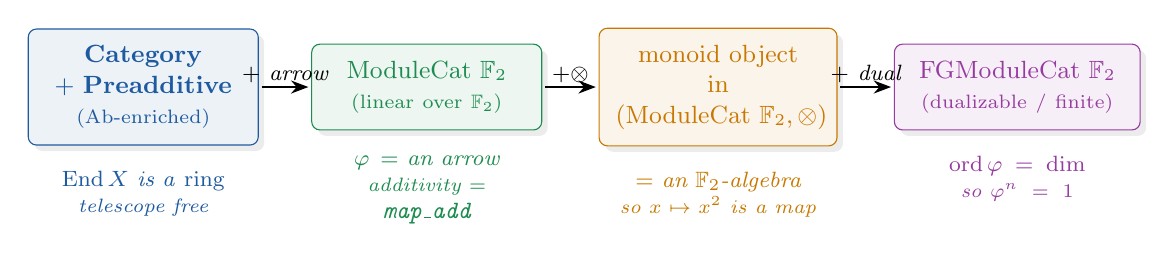
\begin{tikzpicture}[every node/.style={font=\footnotesize}]
  \node[rung,r1,draw=r1,fill=r1!8,text width=2.5cm] (c) at (0,0)
     {\textbf{Category}\\ $+$ \textbf{Preadditive}\\ {\scriptsize(Ab-enriched)}};
  \node[rung,r2,draw=r2,fill=r2!8,text width=2.5cm] (m) at (3.6,0)
     {$\mathrm{ModuleCat}\ \Ff$\\ {\scriptsize(linear over $\Ff$)}};
  \node[rung,r3,draw=r3,fill=r3!8,text width=2.6cm] (o) at (7.3,0)
     {monoid object\\ in $(\mathrm{ModuleCat}\ \Ff,\otimes)$};
  \node[rung,r4,draw=r4,fill=r4!8,text width=2.7cm] (d) at (11.1,0)
     {$\mathrm{FGModuleCat}\ \Ff$\\ {\scriptsize(dualizable / finite)}};
  \draw[ar,thick] (c) -- node[tag,above]{$+$ arrow} (m);
  \draw[ar,thick] (m) -- node[tag,above]{$+\otimes$} (o);
  \draw[ar,thick] (o) -- node[tag,above]{$+$ dual} (d);
  % what each rung buys
  \node[tag,r1,align=center,text width=2.7cm,below=8pt of c]
     {$\End X$ is a \emph{ring}\\ {\scriptsize telescope free}};
  \node[tag,r2,align=center,text width=2.7cm,below=8pt of m]
     {$\varphi=$ an arrow\\ {\scriptsize additivity $=$ \lc{map\_add}}};
  \node[tag,r3,align=center,text width=2.7cm,below=8pt of o]
     {$=$ an $\Ff$-algebra\\ {\scriptsize so $x\mapsto x^{2}$ is a map}};
  \node[tag,r4,align=center,text width=2.9cm,below=8pt of d]
     {$\operatorname{ord}\varphi=\dim$\\ {\scriptsize so $\varphi^{n}=1$}};
\end{tikzpicture}
\end{center}

\begin{center}\small
\renewcommand{\arraystretch}{1.35}
\begin{tabular}{@{}p{0.7cm}p{3.0cm}p{3.5cm}p{4.0cm}p{3.4cm}@{}}
\hline
& \textbf{added axiom} & \textbf{Mathlib category} & \textbf{buys (a theorem)} & \textbf{Lean name}\\
\hline
\textcolor{r1}{1} & Hom-sets abelian, $\circ$ bilinear & \lc{Category} $+$ \lc{Preadditive} & telescope $(\varphi{-}1)\Sigma\varphi^{i}=\varphi^{n}{-}1$ & \lc{telescope}\\
\textcolor{r2}{2} & linear over $\Ff$ & \lc{ModuleCat (ZMod 2)} & $\varphi$ is an arrow; additivity free & \lc{frob}, \lc{frobArrow}\\
\textcolor{r3}{3} & monoidal $\otimes$, monoid object & \lc{MonObj (ModuleCat.of \dots)} & $x\mapsto x^{2}$ is a morphism & \lc{monObj}\\
\textcolor{r4}{4} & has a dual (finite dim) & \lc{FGModuleCat (ZMod 2)} & $\varphi^{n}=1$; $\Tr$ from eval/coeval & \lc{fgObj}, \lc{frob\_pow\_finrank}\\
\hline
\end{tabular}
\end{center}

% ===========================================================================
\section{Rung 1 --- Ab: the telescope is the geometric series}

The \emph{only} axiom is preadditivity: Hom-sets are abelian groups and composition
is bilinear. Then $\End X$ is a ring, and the telescope is \lc{mul\_geom\_sum}. No
field, no characteristic, no finiteness.

\begin{lstlisting}
theorem telescope {C : Type*} [Category C] [Preadditive C] {X : C}
    (@f : End X) (n : @N) :
    (@f - 1) * @s i @m range n, @f ^ i = @f ^ n - 1 := mul_geom_sum @f n
\end{lstlisting}

% ===========================================================================
\section{Rung 2 --- ModuleCat $\Ff$: Frobenius is an arrow, additivity is free}

Work over the base object $\Ff=\lc{ZMod 2}$. The Frobenius $x\mapsto x^{2}$ is an
element \lc{frob} of the endomorphism ring $\Module.\End\ \Ff\ R$; its additivity is
\lc{map\_add} (the freshman's dream, supplied by the module structure). The
endomorphism ring \emph{is} the object's categorical $\End$:

\begin{center}
\begin{tikzcd}[column sep=huge,row sep=tiny]
\End(\lc{ModuleCat.of}\ \Ff\ R) \arrow[r,"{\lc{endRingEquiv}}","\simeq"'] & \Module.\End\ \Ff\ R\\
\lc{frobArrow} \arrow[r,mapsto] & \lc{frob}
\end{tikzcd}
\end{center}

so the Rung-1 telescope, run on the arrow, transports verbatim.

\begin{lstlisting}
noncomputable def frob : Module.End @F R where
  toFun x := x ^ 2
  map_add' x y := by simpa using add_pow_char (R := R) (p := 2) x y   -- freshman's dream
  map_smul' r x := by ...                                            -- @F-linear

lemma frobArrow_telescope (n : @N) :
    (frobArrow - 1) * @s i @m range n, frobArrow ^ i = frobArrow ^ n - 1 :=
  telescope frobArrow n     -- Rung 1, read inside End (ModuleCat.of @F R)
\end{lstlisting}

\begin{note}
\textbf{No field yet.} \lc{frob} is defined for \emph{any} \lc{[CommRing R]
[Algebra (ZMod 2) R] [CharP R 2]}. Additivity is \lc{map\_add}; $\Ff$-linearity is
$r^{2}=r$ in $\Ff$ (\lc{ZMod.pow\_card}).
\end{note}

% ===========================================================================
\section{Rung 3 --- commutative monoid object: why $x\mapsto x^{2}$ is a map}

Make $R$ a \emph{monoid object} of the monoidal category $(\mathrm{ModuleCat}\
\Ff,\otimes)$. Via Mathlib's \lc{MonModuleEquivalenceAlgebra}, monoid objects here
\emph{are} $\Ff$-algebras --- which is precisely what makes squaring a morphism.

\begin{center}
\begin{tikzcd}[column sep=large]
\text{monoid object of } (\mathrm{ModuleCat}\ \Ff,\otimes)
  \arrow[r,"{\lc{MonModuleEquivalenceAlgebra}}","\simeq"'] & \Ff\text{-algebra } R
\end{tikzcd}
\end{center}

\begin{lstlisting}
noncomputable def monObj : MonObj (ModuleCat.of @F R) :=
  ModuleCat.MonModuleEquivalenceAlgebra.inverseObj (AlgCat.of @F R)
\end{lstlisting}

% ===========================================================================
\section{Rung 4 --- dualizable / finite: \lc{Fintype} and $\varphi^{n}=1$ derived}

A finite-dimensional object of \lc{FGModuleCat} $\Ff$ has a right dual. From
\lc{[Module.Finite (ZMod 2) F]} alone, \lc{Finite F}, \lc{Fintype F} and
\lc{CharP F 2} are \emph{derived} --- nothing about counting is assumed:

\begin{center}
\begin{tikzcd}[column sep=large,row sep=tiny]
\lc{Module.Finite}\ \Ff\ F \arrow[r,"{\lc{finite\_of\_finite}}"]
  & \lc{Finite F} \arrow[r,"{\lc{ofFinite}}"] & \lc{Fintype F}\\
\lc{Algebra}\ \Ff\ F \arrow[rr,"{\lc{charP\_of\_inj\_algebraMap}}"] & & \lc{CharP F 2}
\end{tikzcd}
\end{center}

Then the annihilating polynomial $X^{n}-1$ is read off the dimension through a
\emph{monoid map} carrying the algebra Frobenius to \lc{frob}:

\begin{center}
\begin{tikzcd}[column sep=huge,row sep=large]
(F \to_{a}[\Ff] F) \arrow[r,"{\lc{algEndToLin}}","\to^{*}"'] \arrow[d,swap,"{\operatorname{ord}=\dim}"]
  & \Module.\End\ \Ff\ F \arrow[d,"{(-)^{n}}"]\\
\lc{frobeniusAlgHom} \arrow[r,mapsto] & \lc{frob},\quad \lc{frob}^{n}=1
\end{tikzcd}
\end{center}

\begin{lstlisting}
instance : Finite F := Module.finite_of_finite @F            -- from finite dimension
noncomputable instance : Fintype F := Fintype.ofFinite F      -- Fintype DERIVED
instance : CharP F 2 := charP_of_injective_algebraMap ... 2   -- CharP DERIVED

lemma frob_pow_finrank : (frob (R := F)) ^ (Module.finrank @F F) = 1 := by
  rw [frob_eq_frobenius, @L map_pow, @L frob_orderOf, pow_orderOf_eq_one, map_one]
\end{lstlisting}

\begin{note}
\textbf{What stays.} \lc{Field F} remains at Rung 4: a dualizable object of
\lc{FGModuleCat}~$\Ff$ is only an algebra, and $\varphi^{n}=1$ genuinely fails for
non-reduced algebras (e.g. $\Ff[t]/(t^{2})$, where $t\mapsto0$). This is the honest
irreducible core --- but \lc{Fintype} and \lc{CharP} are no longer assumed.
\end{note}

% ===========================================================================
\section{Capstone --- the norm element is a bit}

Telescope $+\ \varphi^{n}=1$ $\Rightarrow$ the norm element $\Sigma_{i<n}\varphi^{i}$
is fixed by $\varphi$, i.e. lands in $\{0,1\}$ --- the ``trace is a bit'', now a
consequence of the object's structure.

\begin{center}
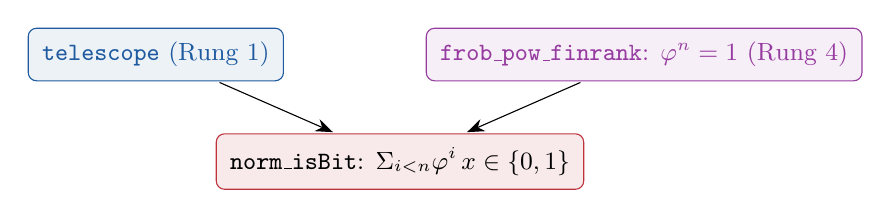
\begin{tikzpicture}[every node/.style={font=\footnotesize},node distance=6mm]
  \node[obj,r1,draw=r1,fill=r1!8] (t) {\lc{telescope} (Rung 1)};
  \node[obj,r4,draw=r4,fill=r4!8,right=18mm of t] (o) {\lc{frob\_pow\_finrank}: $\varphi^{n}=1$ (Rung 4)};
  \node[obj,draw=res,fill=res!10,below=10mm of $(t)!0.5!(o)$] (b)
    {\lc{norm\_isBit}: $\Sigma_{i<n}\varphi^{i}\,x\in\{0,1\}$};
  \draw[ar] (t) -- (b);
  \draw[ar] (o) -- (b);
\end{tikzpicture}
\end{center}

\begin{lstlisting}
lemma norm_isBit (x : F) :
    (@s i @m range (Module.finrank @F F), frob ^ i) x = 0
      @q (@s i @m range (Module.finrank @F F), frob ^ i) x = 1
\end{lstlisting}

% ===========================================================================
\section{Assumed vs.\ derived}

\begin{center}\small
\renewcommand{\arraystretch}{1.3}
\begin{tabular}{@{}p{7.4cm}p{7.2cm}@{}}
\hline
\textbf{classical hypothesis} & \textbf{here}\\
\hline
\lc{[Fintype F]} & \textcolor{r4}{derived} from \lc{[Module.Finite (ZMod 2) F]}\\
\lc{[CharP F 2]} & \textcolor{r4}{derived} from \lc{[Algebra (ZMod 2) F]}\\
additivity of Frobenius (char 2, by hand) & \textcolor{r2}{free}: \lc{map\_add} of the arrow \lc{frob}\\
telescope (bespoke induction) & \textcolor{r1}{free}: \lc{mul\_geom\_sum} in $\End X$\\
$x\mapsto x^{2}$ is a ring map & \textcolor{r3}{structure}: the monoid object \lc{monObj}\\
$\varphi^{n}=1$ (Fermat, cardinality) & \textcolor{r4}{$\operatorname{ord}=\dim$} of the dualizable object\\
\lc{[Field F]} & \emph{kept} --- irreducible (Rung 4)\\
\hline
\end{tabular}
\end{center}

\begin{note}
\textbf{Soundness.} \lc{DobbertinLego/MacLaneLadder.lean} builds \lc{sorry}-free;
\lc{telescope}, \lc{frob\_pow\_finrank} and \lc{norm\_isBit} depend only on
\lc{propext}, \lc{Classical.choice}, \lc{Quot.sound}.
\end{note}

\end{document}
